\chapterimage{Water1.png} % Chapter heading image

\chapter{Water Sources}


\begin{figure}
\begin{center}
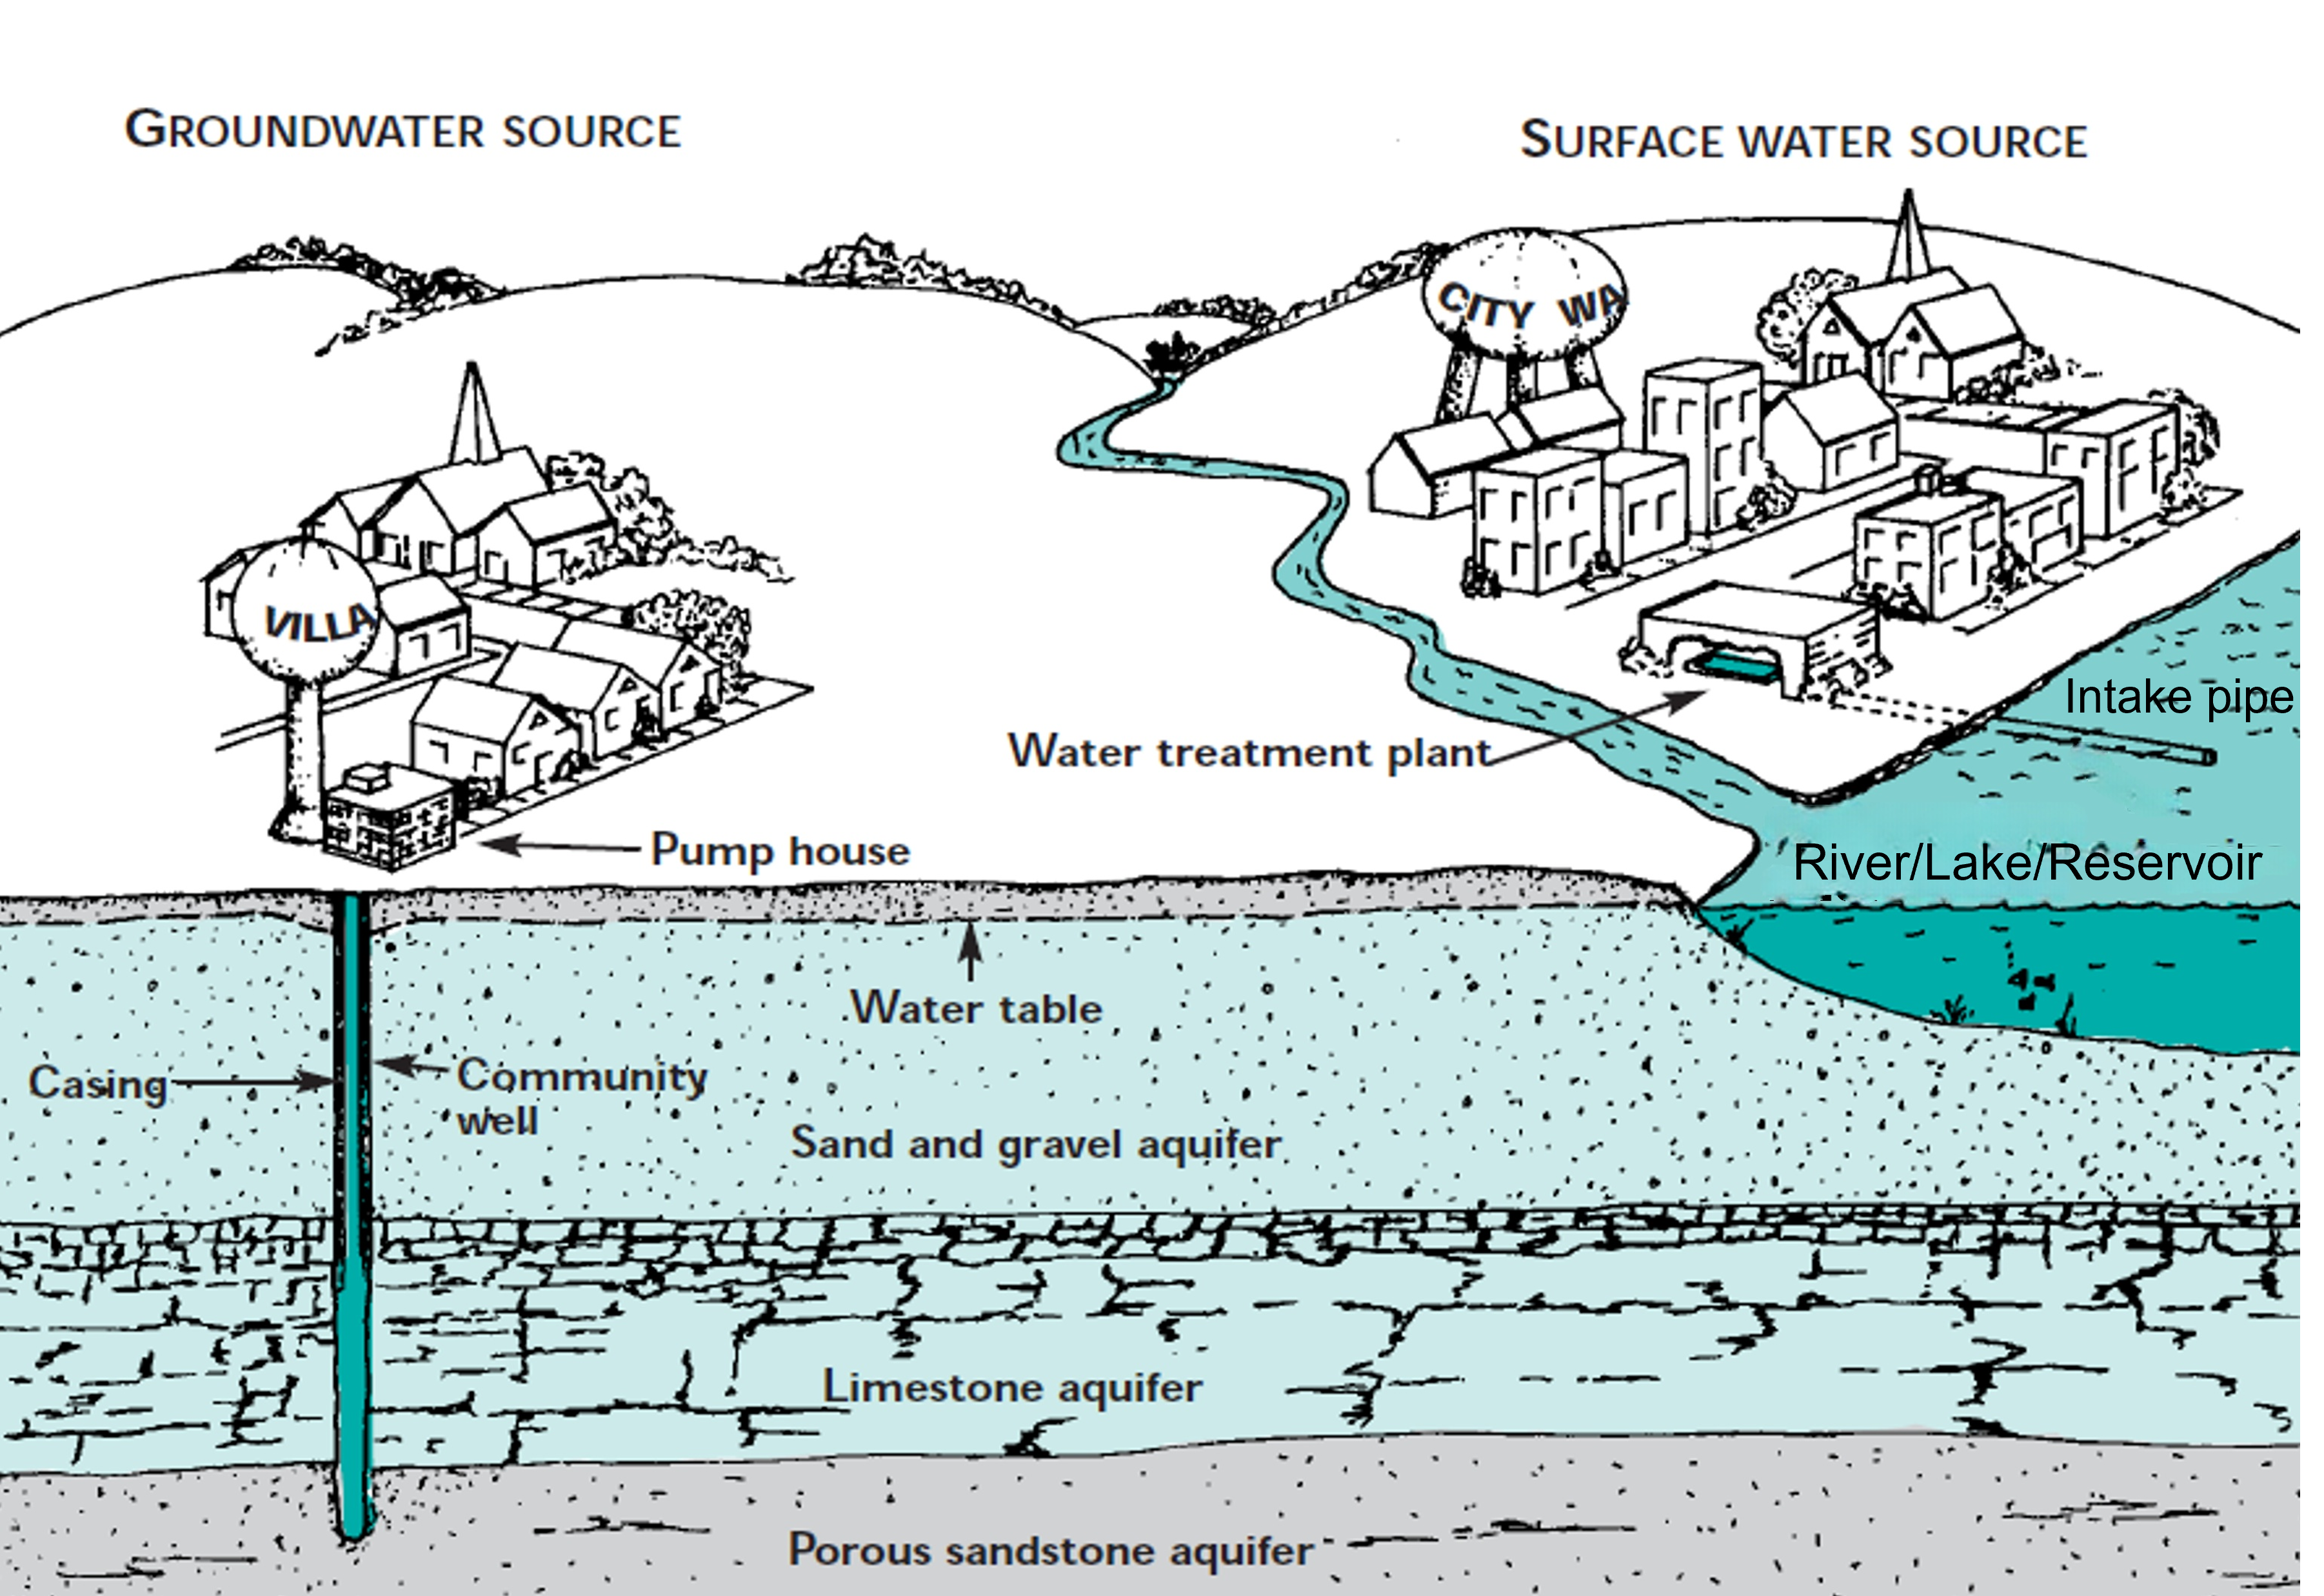
\includegraphics[scale=0.5]{WaterSources}\\
\captionof{figure}{Water Supply Sources}%\caption{}
\end{center}
\end{figure}
\begin{enumerate}
\item Groundwater
\begin{itemize}
\item Groundwater is considered to be water that is below the earth’s crust, but not more than 2500 feet below the crust. Water between the earth’s crust and the 2500-foot level is considered usable fresh water.\\

\item A watershed is an area of land that contributes water to a given location, such as a reservoir, a confluence of two streams, or the ocean. Within a watershed, water from rain or snow flows down the slope, through the soil, or via groundwater flow – and usually by a combination of these routes – to reach the stream and contribute to the flow of the stream. Watersheds are
important sources of drinking water, as well as a habitat for many aquatic species. Healthy watersheds with intact native vegetation and wetlands provide important functions such as water purification, flood control, nutrient recycling, and groundwater recharge.

\item An aquifer is a body of porous rock or sediment saturated with enough groundwater that it can be pumped to the surface and used for drinking water, irrigation, industry, or other uses. . Groundwater enters an aquifer as precipitation seeps through the soil. It can move through the aquifer and resurface through springs and wells.

\item Where groundwater can move rapidly, such as through gravel and sandy
deposits, an aquifer can form.  

\item There are two general types of aquifers: confined and unconfined. Confined aquifers have a layer of impenetrable rock or clay above them, while unconfined aquifers lie below a permeable layer of soil.

\item A common misconception about aquifers is that they are underground rivers or lakes. While groundwater can seep into or out of aquifers due to their porous nature, it cannot move fast enough to flow like a river. The rate at which groundwater moves through an aquifer varies depending on the rock’s permeability.

\item Much of the water we use for domestic, industrial, or agricultural purposes is groundwater. Most groundwater, including a significant amount of our drinking water, comes from aquifers. In order to access this water, a well must be created by drilling a hole that reaches the aquifer. While wells are manmade points of discharge for aquifers, they also discharge naturally at springs and in wetlands.

\item Groundwater can become depleted if we use it at a faster rate than it can replenish itself. The replenishment of aquifers by precipitation is called recharging. Depletion of aquifers has increased primarily due to expanding agricultural irrigation. Groundwater can become contaminated when an excessive amount of pesticides and herbicides are sprayed on agricultural fields, septic tanks leak, or landfills are improperly lined or managed and toxic materials seep through the soil into the aquifer.

\item Aquifers naturally filter groundwater by forcing it to pass through small pores and between sediments, which helps to remove substances from the water. This natural filtration process, however, may not be enough to remove all of the contaminants.

\item Groundwater is obtained from the following:\\
\begin{itemize}
\item Wells
\item Springs that are not influenced by surface water or a local hydrologic event
\item When a well or spring is influenced by an adjacent surface water source or by a local hydrological event, the supply is said to be groundwater under the direct influence of surface water (GUDISW).
\end{itemize}
\item Advantages of groundwater with respect to surface water:\\
\begin{itemize}
\item Groundwater is not as easily contaminated as surface water.
\item The quality of groundwater, while not always as good as would be preferred, is stable throughout the year.
\item Groundwater sources are generally lower in bacteriological count than surface water sources.
\item Groundwater is available in most locations throughout the continental US and Alaska.
\end{itemize}
\item Disdvantages of groundwater with respect to surface water:\\
\begin{itemize}
\item Once a groundwater source is contaminated, it is difficult for it to recover. There is no easy way to remove the contaminants.
\item Groundwater usually contains more minerals than surface water, including increased levels of hardness. Because groundwater is in contact longer with minerals, there is more time to bring them into solution.
\item Removal of groundwater normally requires a pump, thus increasing operation cost.
\item Groundwater is more susceptible to long-term contamination from fuel spills.
\item Groundwater supplies often have high levels of iron and manganese, thus increasing treatment cost and/or causing stains on plumbing and the clothing of customers.
\item Wells in the coastal areas are subject to salt water intrusion into the aquifer20
and well. This contamination is difficult to predict and costly to treat.
\item Sources of contamination can be hidden from sight.
\end{itemize}
\end{itemize}

\item Surface water\\
\begin{itemize}
\item Surface water is water that is open to the atmosphere and results from overland flow. It is also said to be the result of surface runoff 3. These are two ways of saying the same thing.
\item Examples of surface water include:
\begin{itemize}
\item Streams, Rivers, Lakes
\item Man-made impoundments - Reservoirs
\item Wells drilled next to or in a stream or river
\item Rain catchments
\end{itemize}

\item Advantages of surface water with respect to groundwater:
\begin{itemize}
\item It is easily located. It takes no sophisticated equipment to find a surface water source.
\item In many parts of the US, considerable data is available on quantity and quality of existing surface water supplies.
\item Surface water is generally softer than groundwater, which makes treatment much simpler.
\end{itemize}
\item Disadvantages of surface water with respect to groundwater:
\begin{itemize}
\item Surface waters can be easily contaminated with microorganisms that cause waterborne diseases and chemicals that enter the stream from surface runoff and upstream discharges.
\item The turbidity of a surface water source often fluctuates with the amount of precipitation. Increases in turbidity increase treatment cost and operator time.
\item The temperature of surface water fluctuates with the ambient temperature. This makes it difficult to produce consistent water quality at a water treatment plant.
\item The intake structure may become clogged or damaged from winter ice, or the source may be so shallow that it completely freezes in the winter. This is a common problem with surface water sources in the arctic.
\item Removing surface water from a river, lake, or reservoir requires a legal right, referred to as a water right. 
\item Using surface water as a source means that the purveyor is obligated to meet the requirements of the Surface Water Treatment Rule (SWTR) of the State Drinking Water Regulations. This rule requires that, in most instances, any surface water source must have a filtration system.
\item Surface waters that are high in color, especially color that is the result of decaying vegetation, have the potential to produce high levels of Total Trihalomethanes (TTHM). These chemical compounds are formed when chlorine is added to the water. The problem with the TTHM is that some of them are carcinogenic (can cause cancer) and are referred to as disinfection by-products (DBP).
\end{itemize}
\end{itemize}
\end{enumerate}


An artesian well is a well that taps into a confined aquifer (see above). Under artesian pressure, water in the well rises above the top of the aquifer, but does not necessarily reach the land surface. A flowing artesian well is one that has been drilled into an aquifer where the pressure within the aquifer forces the groundwater to rise above the land surface naturally without using a pump. Flowing artesian wells can flow on an intermittent or continuous basis and originate from aquifers occurring in the either unconsolidated materials such as sand and gravels or bedrock, at depths ranging from a few meters to several thousand meters. All flowing wells are artesian but not all artesian wells are flowing wells.